\chapter{Editing}
There are three types of objects which can be exported as mdl: Empties,
Meshes and Lamps. Other objects like curves and surfaces will have to be
converted to meshes before attempting to export them.

\section{Empties}
Empties appear in mdl files as Dummies. Like in blender they are used to group
objects. In addition there are special types of Empties/Dummies which for
example indicate locations for spells effects.

\subsection{Dummy}
Simple Empties with a parent are either used to group objects or
indicate a special location for the engine. If a Dummy doesn't have a
parent it is considered to be a Rootdummy instead of a simple Dummy
and the available options will change. \\

\begin{figure}
  \centering
  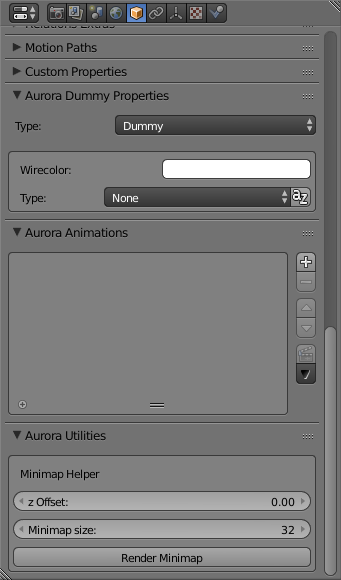
\includegraphics[trim=0 0 0 0, clip, width=0.33\textwidth]{panel_dummy}
  \caption[panel dummy]{Dummy Property Panel}
  \label{fig:panel_dummy}
\end{figure}

The following types of Dummies are available:
\begin{description}[leftmargin=6em,style=nextline]
    \item[None] Simple dummy without any special purpose.
    \item[Ground] Indicates the ground level for spells/ visual effects
    \item[Impact] Impact target for most spells/ visual effects.
    \item[Head Hit] Spells/ visual effects
    \item[Head] Head location for Spells/ visual effects
    \item[Hand] Point of origin for (some) spells. If a spell/ visual is originating from this mdl, this will be the point of origin most of the time.
    \item[Use 1] Use Node for placeables or doors. Upon receiving a use command a character will move to the closest of the two use nodes.
    \item[Use 2] Use Node for placeables or doors. Upon receiving a use command a character will move to the closest of the two use nodes.
\end{description}
Neither of the special Dummys are mandatory. If a particular Dummy is
missing from the mdl, the engine will use (0,0,0) as the default location
for that Dummy. \\

Selecting the dummytype is not enough to make them work, they need to have
the correct name or to be precise the suffix.
The export script will try to generate a valid name depending on
the Dummys type, but it is recommended to do it manually to avoid naming
conflicts. \\

You can use the button next to the Dummytype selector to generate a
working name. It will take the dummy's name and append the needed suffix for
the selected Dummytype. \\

\subsection{Rootdummy}
Each mdl requires at least one Empty: The Rootdummy. All children
of this Rootdummy are considered to be part of the same mdl. \\

An Empty with the type Dummy and without a parent will automatically be
considered a Rootummy. The Rootdummy must have the same name as the
mdl file (minus the file extension). Rootdummys hold additional
information about the model and the Aurora Property panel will
change accordingly.

\subsubsection*{Classification}
\begin{description}[leftmargin=6em,style=nextline]
    \item[Item] Any inventory item.
    \item[GUI] Unknown.
    \item[Effect] For visual effects.
    \item[Door] Doors, be it generic or for tilesets.
    \item[Character] Creature or placeables. 
    \item[Tile] For tilesets.
    \item[Unknown] Avoid using this. It may be set during import.
\end{description}

\subsubsection*{Supermodel}
Reference to another mdl file. All animations from that file 
will be available in this mdl.

\subsubsection*{Animationscale}
Unknown

\subsection{Reference Node}
The purpose and usage of these nodes is unknown. Supposedly it can be used to
reference other mdl files. These nodes can be found in some spells and
most of the time references fx\_ref.

\subsection{Patch Node}
The purpose and usage of these nodes is unknown. They occur in some spells, but
they seem to behave exactly like normal dummy nodes, i.e they have the same
attributes.

\section{Meshes}

\subsection{Trimeshes}
The default type of mesh consisting of triangles. It is not necessary to convert 
the faces to triangles, the export script will handle that.

\subsubsection*{Wirecolor}
This is unused in-game. You can safely ignore it. This probably defines the
color for the object's wire-frame in 3dsmax.

\subsubsection*{Self-Illumination Color}
Makes the mesh seem to glow. It does not act as a light source however.
This will not be visible in blender's viewports or renderers.

\subsubsection*{Ambient Color}
OpenGL material property. The Aurora Engine uses per-object ambient light,
which you can define here. Blenders ambient light is defined on a per scene
basis. Therefore this property not be visible in blender's viewports or
renderers.

\subsubsection*{Shininess}
A matching .txi file for the texture and a .env file are necessary

\subsubsection*{Tilefade}
Only available for tiles. Controls whether this mesh will turn invisible to
clear the view.
\begin{description}[leftmargin=6em,style=nextline]
    \item[None] This mesh will always be visible.
    \item[Fade] The object will fade.
    \item[Base] Unknown
    \item[Neighbour] The object will fade along with meshes in neighbouring tiles.
\end{description}

\subsubsection*{Render}
Controls whether this objects should be rendered in-game. Meshes can still
cast a shadow without being rendered.

\subsubsection*{Shadow}
Controls whether this objects should cast a shadow.

\subsubsection*{Beaming}
Unknown. Probably unused.

\subsubsection*{Inherit Color}
Unknown. Probably unused.

\subsubsection*{Rotatetexture}
Only available for tiles. Auto-Rotates textures so the UVs are rotated
the same way to avoids seams between tiles.

\subsubsection*{Transparencyhint}
Helps the engine to prioritize transparent meshes, similar to a z-buffer. If
you have multiple meshes with transparent textures and have issues like
flickering try changing this value.

\subsubsection*{Smoothgroup}
Controls how or whether at all to create smoothing groups or shading groups.
\begin{description}[leftmargin=6em,style=nextline]
    \item[Separate] Each face will have its own smoothing group. This results in no smoothing at all.
    \item[Single] All faces belong to a single smoothing group. Meshes will be smoothed.
    \item[Auto] Auto generate smoothing group, depending on the settings in blender and edges marked as sharp. Replicates blenders smoothing as closely as possible.
\end{description}

\subsection{Danglymeshes}
Danglymeshes are Trimeshes which are"bouncy" or "dangly". They are affected by
wind, character movement and spells. A danglymesh has a set of weights which
determine how far a vertex can be displaced from its original position.

A Danglymesh has the following properties in addition to the properties of a 
trimesh:
\begin{description}[leftmargin=6em,style=nextline]
    \item[Dangle group] The dangle group is a vertex group containing the weights of vertices for the danglymesh. You must select an existing vertex group.
    \item[Period]
    \item[Tightness]
    \item[Displacement]
\end{description}

\subsection{Skinmeshes}
\todo{Skinmesh description}
A Skinmesh has the following properties in addition to the properties of a 
trimesh:
\todo{List properties}

\subsection{Animeshes}
Animeshes are Trimeshes with animated UV textures. At the moment Animeshes
are imported as Trimeshes and will thus lose their animations.

An Animesh has the following properties in addition to the properties of a 
trimesh:
\todo{List properties}

\subsection{Walkmeshes}
Walkmeshes indicate where a character can walk. It is necessary to select 
the appropriate type of walkmesh, which depends on the type of model itself. 
The following types are available:
\begin{description}[leftmargin=10em,style=nextline]
    \item[Tileset] Walkmesh for tiles. Assign Materials to each face to set the
                   surface type of tile (stone, grass, unwalkable, ...).
                   This will also affect footstep sounds and grass growth.
    \item[Door: Closed] The walkmesh for the closed state of a door. Blocks movement.
    \item[Door: Open 1] The Walkmesh for the first open state of a door. Blocks movement.
    \item[Door: Open 2] The Walkmesh for the second open state of a door. Blocks movement.
    \item[Placeable] Walkmesh for placeables. Blocks movement.
\end{description}

\section{Emitters}
Support for Emitters is rudimentary. Blenders particle systems is too
different to allow a direct import, instead Emitters are imported as plain
text. While all data will be retained, editing is difficult.

\section{Lamps}
Blender lamp properties will be used for exporting a light.
Exported properties are:
\begin{itemize}
\item Color
\item Distance
\end{itemize}

\subsection*{Light type}
There are some special light types, all of which are used to give builders
the ability to select light color in the Toolset.
\begin{description}[leftmargin=8em,style=nextline]
    \item[Mainlight 1] For Tiles only. Color can be changed in the Toolset.
    \item[Mainlight 2] For Tiles only. Color can be changed in the Toolset.
    \item[Sourcelight 1] For Tiles only. This is actually a burning flame. Color can be changed in the Toolset.
    \item[Sourcelight 2] For Tiles only. This is actually a burning flame. Color can be changed in the Toolset.
    \item[Default] Default type, can always be used. Blenders lamp properties will be used (color and distance)
\end{description}

\subsection*{Wirecolor}
This is unused in-game. You can safely ignore it. This probably defines the
color for the object's wireframe in 3dsmax.

\subsection*{Priority}
Unknown. Might control when the light source casts a shadow.

\subsection*{Ambient Only}
This controls if the light is only an ambient light source or
if it is directional as well.

\subsection*{Fading}
Unknown. Might activate some kind of distance fall off for the light.

\subsection*{Shadows}
Determines if this light is capable of casting shadows.

\subsection*{Is Dynamic}
Unknown.

\subsection*{Affect Dynamic}
This controls whether this light affects dynamic objects, i.e. characters.
Disabling this will prevent this light from casting shadows with dynamic
objects, but it will in turn improve performance.

This is basically a less strict version of the \textit{Shadows} setting.

\subsection*{Lensflares}
Add a series of lens-flares for this light.

Lens-flares are unavailable for Mainlights or Sourcelights.
\begin{description}[leftmargin=6em,style=nextline]
    \item[Texture] Texture for this flare
    \item[Colorshift] Unknown. Possibly color difference from the light color.
    \item[Size] Size of the flares. This will scale the texture.
    \item[Position] Distance from the lights origin.
\end{description}

\section{Materials \& Textures}
\begin{description}[leftmargin=6em,style=nextline]
    \item[Diffuse] TODO
    \item[Specular] TODO
\end{description}

\subsection*{Alpha}
TODO

\section{Animations}

\begin{itemize}
    \item Location
    \item Rotation
    \item Scale (Uniform only)
    \item Material or Texture Alpha
\end{itemize}